\documentclass[12pt]{article}
\usepackage{bashful}
\usepackage[affil-it]{authblk}
\usepackage{times}
\usepackage{geometry}
\geometry{
a4paper,
total={170mm,257mm},
left=20mm,
top=20mm,
bindingoffset=8mm
}
\usepackage[colorlinks=true,citecolor=blue]{hyperref}
\usepackage[comma]{natbib}
\bibliographystyle{agsm}
\usepackage{setspace}
\linespread{1.25}
\usepackage{imakeidx}
\usepackage{graphicx}
\makeindex[columns=3, title=Alphabetical Index, intoc]
\renewcommand{\contentsname}{Table of Contents}
\usepackage{multicol,lipsum}


\title{
\vskip Predicting the success rate of startups in India and their ability to survive a global crisis using machine learning
\includegraphics[scale=0.9]{Figures/SETU_Final.png} 
}
\author{}
\date{}

\begin{document}

\bash
texcount -sum -1 main.tex 
\END 

\maketitle  
\begin{center}
    \begin{flushleft}
    STUDENT NAME:\space Priyanka Jiddigere Venkatesh
    \bigbreak
    STUDENT NUMBER:\space C00290849
    \bigbreak
    COURSE NAME:\space Master of Science in Data Science
    \bigbreak
    DEPARTMENT:\space Department of Computing and Data Science
    \bigbreak
    COURSE CODE:\space KCDAR\_M\_Y5
    \bigbreak
     WORD COUNT:\space \emph{\bashStdout}
    \bigbreak
    SUPERVISOR:\space Dr. Jason Barron
    \bigbreak
    DATE OF SUBMISSION:\space \date{\today}
    \end{flushleft}
\end{center}  


%TC:ignore

\newpage
\vfill\noindent
\begin{center}
  \textbf{DECLARATION}
\end{center}

* I declare that all material in this submission is entirely my own work except where duly acknowledged.

* I have cited the sources of all quotations, paraphrases, summaries of information, tables, diagrams, or other material; including software and other electronic media in which intellectual property rights may reside.

* I have provided a complete bibliography of all works and sources used in the preparation of this submission.

* I understand that failure to adhere to the Institute's anti-plagiarism policies is a serious offense.

\vspace*{20em}\noindent


Student Name:\space\space\space\space Priyanka Jiddigere Venkatesh
\bigbreak
Student Number: C00290849
\bigbreak
Signature:
\bigbreak
Date:\space\space\space\space\space\space\space\space\space\space\space\space\space\space\space August 15, 2023

\vspace*{4em}\noindent

\newpage
\begin{center}
  \textbf{ACKNOWLEDGEMENTS}
\end{center}

I want to acknowledge the kind support and assistance of all the people who have helped me complete this research successfully. 

First and foremost, I would like to express my respect and gratitude to my supervisor, Dr.Jason Barron for his mentorship and guidance throughout this study.

My heartfelt gratitude also goes to the staff and lecturers from the Department of Computing at the SETU Carlow Campus for helping me gain more knowledge and improve my skills to reach this level. 

I also wish to acknowledge the support and motivation of my peers throughout the thesis process.

And finally, I would like to express my special gratitude to my friends and family for their constant encouragement to stay focused and complete this study successfully.

\newpage
\begingroup % start a TeX group
\color{black}% or whatever color you wish to use
\hypersetup{linkcolor=black}
\tableofcontents
\endgroup 

\newpage
\hypersetup{linkcolor = black}
\listoffigures

%TC:endignore

\newpage

\section{INTRODUCTION}
India, one of the world's fastest-growing economies, has undergone significant economic changes over the past few decades. The country's economic landscape has experienced significant shifts and has witnessed substantial growth, transforming it into the world's sixth-largest economy by nominal GDP. India is known for its diversity in all fields as witnessed by the many sectors of industries, technology, and healthcare to name a few. Circling back to technology, India soon caught up on the technological advancement and has been a significant contributor to the country’s economic growth. The establishment of several home-owned technological companies put India on a fast track, Especially with the emergence of startups, the whole dynamic changed with many startups emerging successfully and contributing to the country’s economic growth.
The Indian startup ecosystem was surprisingly thriving during one of the global crises that shook the world, the Pandemic, proving that it has resilience and adaptability. Despite all the challenges faced, startups have been a pillar of great innovation and flexibility in their approach. The closure of brick-and-mortar businesses led to an increase in remote work opportunities. Moreover, there has been a noticeable shift in consumer behavior, which led to the boom of digital transformation. Indian startups have been able to tackle these challenges head-on by pivoting their business models, developing digital solutions, and embracing new technologies. With the support of government initiatives and financial assistance programs, the future looks brighter. The government of India's 'Make in India' initiative has emerged successfully, recognising 26 startups daily by DPIIT (Department for Promotion of Industry and Internal Trade) \citep{singh2020analyzing}.

The pandemic, is the gift that keeps on giving or not. As the world grappled with the chaos and the uncertainty, so did the whole startup ecosystem. But, they were a tough bunch and also were a brave soul to fight this pandemic. The startups who were new to the market did not fear at all, they were able to utilize this curse by measuring and analyzing the pandemic that also brought opportunities with it. With remote work becoming the new norm, startups were able to embrace the change with open arms. Suddenly, the whole world became their oyster, or should in a single word it could be said that their Zoom meeting. This new norm was able to connect and bring up new people thus breaking up barriers,

The Indian start-up ecosystem has been able to prove that they are incredibly resilient in the face of the pandemic, they are able to thrive through the challenges that were created during the crisis. Start-ups 
were able to demonstrate adaptability and bring up an innovative edge by pivoting their business models to align with changing consumer behaviour, placing an emphasis on the massive digital transformation. Brick-and-mortar businesses suffered greatly, but Indian start-ups were able to 
embrace the remote work opportunities and the culture associated with them and bring up digital solutions for their products and services. The Indian government has also played a crucial role in supporting start-ups during this time by introducing financial assistance programs and other 
initiatives that were able to greatly contribute to the overall success of the start-up ecosystem. 

In recent years, India has been able to emerge as a global hotspot for entrepreneurship and business innovation. The start-up culture in the country has really got a major boost with a growing number of entrepreneurs and investors who are now recognizing the immense potential and opportunities that Indian Startup Culture has to offer. The thriving startup ecosystem also has been able to attract talent from all over the world, leading to a highly diverse and dynamic business environment.
One of the key factors that has a major contribution to the rapid success of Indian startups is the availability of in-house skilled and talented professionals. The country has a large and diverse pool of young and educated individuals who are eager to contribute to this constructive growth and 
development of these innovative ventures who have the primary goal of shaping the country's vision in a positive direction. This talent pool is now coupled with the advancements of the technologies and digital infrastructure that are able to facilitate the rapid growth of Indian startups. 
Another significant factor that has an important role in the growing success for Indian startups is the extensive support that is provided by the government and the various financial institutions. From offering tax incentives and lower taxation in the initial growth stage mainly providing access to the capital, the government has also created a favorable environment for startups so that they could thrive. 
Moreover, financial institutions have been able to play a crucial role by providing funding and investment opportunities to startups. The success of Indian startups can also be attributed to their ability to adapt and go through a continuous process of innovation so that they are able to face any sudden challenges that might come up in the future. The COVID-19 pandemic had created numerous obstacles for businesses to grow worldwide, but Indian startups were able to quickly adapt to these unwanted situations and find solutions. Many of the startups shifted their operations online by leveraging the new robust technology so that they are able to continue serving their customers.

There was a massive change in consumer behavior? Well, let's now talk about this plot twist! As people adapted to the "new normal," their preferences and habits started to shift in a positive direction. Demand for specific products skyrocketed, while others, fell face-first into a giant pothole. And also to support the whole change let's not forget the rise in digital transformation. Startups that were already on the rise of the digital bandwagon had a huge head start, leaving the rest of the pack in their virtual dust. From the installation and adaptation of contactless payments to online shopping, the digital realm became the superior knight in shining armor, minus the clunky armor and medieval jousting. As this Startup Culture grows in the future, the prospects for Indian startups are very promising. The resilience and adaptability that they have shown in the time of any pandemic situation which was quite challenging for every business model have helped them to grow in the long term and achieve their desired success creating much more opportunities in the future. Thus, with the continuous support of the government along with the relentless drive of entrepreneurs, the Indian startup ecosystem has been able to move faster towards positive achievements in the years to come. At the peak of this pandemic, the Indian startup ecosystem has been able to emerge as the beacon of hope for many. The ability of these Indian startups to adapt and evolve with the rising difficult solutions in this phase of adversity has been nothing less than a remarkable approach. They have not only survived but also thrived in a time when most of the traditional home-grown businesses have struggled to stay afloat in the market and have also been profitable in the time of the pandemic.

\newpage
\section{PROBLEM STATEMENT}
While starting a new business venture is always interesting and exciting. Regardless of the field of business, it is imperative that entrepreneurs consider a lot of factors and do a lot of research before venturing into the said business. Starting a business demands not just having a big-picture perspective but also having a thorough awareness of the many different variables that affect how well it does. Entrepreneurs must carefully weigh a wide range of factors before starting a business because the environment is influenced by economic, social, and geopolitical factors. Additionally, the recent spike in worldwide crises, such as wars, pandemics, and recessions, has highlighted the significance of resiliency and adaptation in the face of unforeseen difficulties.

Factors such as market analysis, target audience identification, financial feasibility, competitive landscape, and regulatory considerations play crucial roles in shaping a startup's prospects. Conducting comprehensive market research enables entrepreneurs to discern gaps and opportunities, while also identifying a clear value proposition ensures that a business meets customer needs. Understanding the competitive landscape aids entrepreneurs in positioning their businesses effectively. Moreover, compliance with legal and regulatory frameworks is also vital to avoid potential pitfalls.

Among the many unforeseen circumstances, a crisis on a large scale or a potential global crisis could alter the course of businesses. Global crises like recession, the pandemic, or wars and geopolitical tensions could disrupt the entire business dynamic. Although India didn't experience substantial occurrences of recessions and wars, the global crisis that had a profound impact on the nation was undoubtedly the COVID-19 pandemic. Numerous well-established enterprises succumbed suddenly, while many others managed to endure the pandemic due to their unwavering resilience and ability to adapt swiftly.

\subsubsection{Research Question}

\begin{enumerate}

\item Can machine learning models get employed to make a prediction on the success rate of startups in India and check their ability to survive a global crisis like the COVID-19 pandemic or economic recession?  

\item How much has the COVID-19 pandemic contributed to the growth of startups in India, as measured by the percentage increase in the total funding raised by startups during the pandemic compared to the previous years?

\end{enumerate}

\subsubsection{Research Objectives}

There are several key objectives have been associated with the assessment and a detailed discussion has been provided on the key objective of this assessment. 

\begin{itemize}

\item Develop a robust predictive model: It is the primary objective of this research, where the main focus is to develop a reliable predictive model that can help to find the probability for startups that are based in India. To achieve the result, it will use the data from before and after COVID-19, and advance machine learning techniques to make an accurate prediction. 

\item To find key indicators of resilience: The study will also try to highlight the main factors that play a significant role in the success of a startup and its ability to withstand situations like pandemics and recessions. Understanding these factors will contribute to deriving proper strategies that can help startups to overcome such situations in the future. 

\item To offer valuable insights: In the way of achieving its key objective, the research will provide valuable insights to policymakers, investors, and entrepreneurs. By the analysis of this research paper, they will be able to take well-informed decisions while they fund or get associated with any startup. The policymakers can further design and implement such policies that can provide support to startups in rough times like pandemics and recessions. 

\end{itemize}

\pagebreak
\section{LITERATURE REVIEW}

\subsection{Chapter overview}
According to \citep{jain2016growth}, there is no clear definition for a startup in the Indian context and the whole startup dynamic depends on a number of factors."Startup India, Standup India" was started in India in 2016 by then Prime Minister to boost the country's entrepreneurial growth and many incentives were offered to develop the same \citep{jain2016growth}. 

\subsection{Definitions and Characteristics of A Startup}
Analyzing the report stated by \citep{sreenivasan2023modelling}, a crucial starting point for understanding organizational resilience in startups is to define what constitutes a startup and its identity and distinct characteristics. Startups are creative, youthful businesses that are usually just starting and are looking to establish and test a scalable business plan. Startups differ from established firms in that they have the potential for fast development, are risk-takers, and are quick to adapt to changing market conditions. Since startups attempt to deliver new goods, services, or business models to the market, the notion of startups is frequently linked to disruptive innovation. The author here also emphasizes the importance of the “Lean Startup” methodology, practicing this approach makes a startup company able to adopt a systematic process relating to experimentation and validated learning to identify and refine the business model.  The “Build-Measure-Learn” feedback loop is the core of this approach as it allows the organization to collect feedback on the goods and services provided by them to the customer and analyze the feedback to refine the identified drawbacks and mistakes, and this identical approach establishes a market fit for the product as it ensures that the product is a final attempt of the company or the organization to address all the concerns and expectations of the customers. 

According to \citep{raj2022developing}, Startups are frequently distinguished by their few resources and the requirement to use creativity to overcome challenges. The existence of startup companies rotates around in a fast-growing environment, market uncertainties, changing customer demands, and emerging trends. The adopted approach to counter the barriers of the market eventually turns out to be the call for their success and failure in the market, ultimately their ability to respond to the unexpected events in the market can determine their success and survival in the market. For presenting an impressive and impactful report detailing or investigating the position of the startup in a crisis like the Covid-19 pandemic. The presence of adversity is vital in organizations looking to establish themselves as successful startup as the approach and focus on validating their business model through continuous learning aligns with the concept of resilience as the capacity to adapt and recover. Therefore, the continuation of the happening of the unexpected event in the lifespan of the startups as they have to face many times events that are unforeseen, enhances their ability to pivot, innovate, and respond, which normally becomes crucial in ensuring their survival and sustainability.

In the research conducted by \citep{raheja2023machine} Altogether, it can be estimated that startups are dynamic in nature and innovative ventures that operate in an environment of uncertainty and change. They are a fascinating and important subject for research in the context of organizational resilience during crises like the Covid-19 epidemic because their emphasis on experimentation, verified learning, and adaptation matches the fundamentals of resilience. 

\subsection{Factors influencing startup success and failures}
\citep{zhang2022startups} has provided an explored study in his analytical report that a strategy of starting a new firm startup has been widely adopted around the globe and also because luring has just not seasoned company owners but also at the same time recent graduates looking for challenges. Universities nowadays provide meaningful courses to meet the demands of the students. The basic motive of building a strong and impactful startup is generating a high return on the invested amount. And it is important to admit the data that reflect the growth in the rate of startup in India and the same is the case for the percentage of failures in startup across the Indian Market, it can be addressed by evaluating the reason behind only 40\% of the startups making a profit in the current market. The disorganized and fragmented nature of Indian markets makes it difficult for startups to prosper. Every 30 to 50 kilometers, Indian customer behavior varies, making it extremely challenging for
startups to develop a generalised business or marketing strategy for their goods or services. The majority of startups tend to stagnate and eventually fold \citep{sharma2019challenges}. And numerous factors are associated with the chances of failure, this segment of the report aims to provide an impressive analysis of the factors that are directly responsible for influencing the success and failures of a business start-up.  In short, the main factors include access to adequate funding, the quality of the management team, product-market fit, adaptability, innovation, and the ability to navigate market dynamics effectively. Success for startups can be broadly divided into two categories, despite the fact that there is no one particular definition or route to it. A corporation may choose to do an IPO (Initial Public Offering), in which case its shares are available for sale to the public and the company is listed on a public stock exchange. Another is merging with or being acquired by another company (M\&A), in which the startup’s founders or investors receive fast cash in exchange for their stock, also called an ”exit
strategy” \citep{bangdiwala2022predicting}.

\cite{zhimeng2021assessing} in his study addressed that Covid-19 has brought up numerous challenges in terms of start-ups, exacerbating their already precarious position. The COVID-19 epidemic has caused severe disruptions in the world economy, with extensive lockdowns and social isolation measures having an impact on businesses, especially those that are just getting started. Startups that significantly rely on loans and finance to maintain their operations face enormous hurdles as a result of these negative repercussions. Accessing crucial capital for companies has become more challenging because of the pandemic's financial difficulties. In addition to financial difficulties, COVID-19 has also shaken entrepreneurs' confidence, slowing the expansion of new businesses. For startups, the fear of failure has become a powerful barrier that makes it more difficult for them to survive these difficult times. The disruption of supply chains has also made it more difficult for startups to endure and grow. Despite the difficulties, several chances have emerged, particularly in pandemic-related industries including vaccine development, healthcare, and distant communication, providing growth prospects. \citep{wagh2022study} in their article have published that startups are looking for alternate tactics to maintain their survival as they are compelled to change.

This study by \citep{wagh2022study} further intends to investigate the direct association between the number of daily new COVID-19 cases and startup investment. To check for any cointegration connections between the variables, traditional regression models will be used in Excel and Stata programming. By focusing on this important topic, the study aims to provide insightful information that will help entrepreneurs and policymakers alike navigate these uncharted waters and assist the survival and resilience of businesses both during and after the epidemic.

\subsection{Machine Learning in Predictive Modeling}
The study conducted by \cite{sujath2020machine} mainly aimed at the application of machine learning to predictive modeling for startups during and after the Covid-19 pandemic. Support vector machines, decision trees, random forests, and neural networks are just a few examples of machine-learning algorithms that have demonstrated significant promise in the analysis of massive datasets and the discovery of patterns that might be a sign of a startup’s likelihood of surviving crisis like the Covid-19 epidemic. Startups faced exceptional difficulties as a result of the Covid-19 pandemic, particularly the ones that were just getting started. Startups’ capacity to obtain capital and successfully negotiate market dynamics has been greatly damaged by widespread lockdowns, social segregation policies, and interruptions in global economic activity. The fear of failure grew to be a significant obstacle for new businesses, and many companies experienced financial hardship as getting loans and funding got more and more challenging. Even Nevertheless, opportunities for companies working in pandemic-related sectors including healthcare, vaccine development, and remote communication appeared among the difficulties, demonstrating the flexibility and adaptability of entrepreneurs in emergencies.

According to \citep{varma2023restarting}, Machine learning algorithms have been essential in this situation in helping businesses anticipate and manage their chances of survival both during and after the pandemic. These algorithms can forecast patterns and possible outcomes for startups by examining past data, allowing business owners and investors to make well-informed choices. To determine a startup's probability of success during the pandemic and beyond, machine learning algorithms may evaluate a variety of parameters, including availability to capital, product-market fit, management team quality, and flexibility. For instance, machine learning techniques have been used to forecast how COVID-19 may affect the income and growth trajectories of startups, assisting business owners in creating effective crisis management plans. Machine learning algorithms may give entrepreneurs insightful information about prospective possibilities and obstacles in their target markets by analyzing data on COVID-19 cases, economic indicators, and industry trends. Additionally, these prediction algorithms have been used to locate possible pandemic-related industry areas where entrepreneurs may prosper. Startups can strategically modify their goods or services to meet new market demands by analyzing the pandemic's effects on various industries and spotting emergent wants.

As per \citep{verma2022machine} Adding more machine learning models has been crucial in forecasting how sociodemographic characteristics may affect the frequency of COVID-19 in various countries, giving entrepreneurs crucial information to target certain markets or modify their operations appropriately. It is important to recognize that complete and reliable data are necessary for the successful application of machine learning in startup predictive modeling. It can be difficult to collect and organize data in the quickly shifting circumstances of a pandemic. Additionally, machine learning model interpretability is also a crucial factor to take into account, particularly in delicate industries like healthcare where openness and clarity are crucial. During and after the Covid-19 pandemic the incorporation of machine learning in predictive modeling for startups has shown promising outcomes in determining survival chances in assessing survival prospects and identifying opportunities along with assisting entrepreneurs and investors in making informed decisions. As data continuous to play an important role in the adoption of machine learning techniques in the startup ecosystem is likely to grow, thus empowering the startups to encounter the uncertainties and create a strong base at the same point of time to handle the smooth workflow at the times of occurrence of the crisis. 
\citep{mukul2023innovative} in his research evaluated that it is important to utilize both machine learning and human expertise for producing and maintaining a good quality of decision-making and ensuring the successful expansion of the startup in the modern era. 

\subsection{Startup Ecosystem in India}
As per \citep{parthasarathy2022decision}, India is a vast and very rapidly growing country so its products and services requirements are also very big, during the time of COVID-19 the supply chain of a lot of products has been cut off which has created a shortage of lots of products and services in the Indian market. And a lot of startups in India have identified this shortage as an opportunity for them to establish their name. This has contributed to providing growth for the ecosystem of startups in India, along with this there is a lot of help is also provided by the government of the country so that the entrepreneurs get encouraged. The paper provided by \citep{eliganurstudy}, highlights how the growth in the Indian startup ecosystem has resulted in creating new job opportunities in the country, the paper also studies the impact of factors like talent development programs, incubators, and accelerators on the startups of India and how it has promoted the growth for the startup companies and provided new solutions in the process of employment generation. At the end of the paper, the researchers have also mentioned how the accessibility to finance and government support through policies has facilitated the expansion of entrepreneurs, ultimately leading to more job opportunities being created. Among the many measures provided are financial support for incubators, the creation of innovation centers, tax breaks, and a streamlined business registration  \citep{korreck2019indian}. The startup environment in India is constantly changing, which attests to its adaptability and tenacity.

As per the research conducted by \citep{shah2023study}, the authors have mentioned in their paper that in recent times India has emerged as a leading point for startups, the government of India has come up with a lot of new policies and initiatives which has not only created opportunities for the startups that are based on India but also from the world. The paper provided by the author emphasizes the impacts of policies like Startup India, the Fund for Funds for Startups, and the 'Atal Innovation Mission' and how these initiatives have boosted the morals of Indian startups. In the paper, the authors have also listed the key factors that are attracting most of the startups, such as the country provides a large and ever-expanding market to sell the products and services, the startup companies can get a lot of talented employees for them on a cost-effective price, the policies and benefits provided by Indian government also act as a catalyst in the process, and the findings are easily available for the Startups. The authors have concluded the paper by listing the challenges that startups have to face in India. 

Another author \citep{yadav2021impact}, has researched understanding the impact of COVID-19 on different entrepreneurial schemes that were running in the country, in the report the author mentioned that Indian startups were trying to grow by the means of the aid that were recently introduced to them in the face of government startup supportive policies. According to the author India was termed the fastest-growing economy in the world before COVID-19 stuck the world economy, but the spread of COVID-19 has made a turnover in the pathway of the country, in the paper the author has highlighted that India was on a way setback from the year 2018 because of the global recession and effects of COVID-19 has a acted as a catalyst to take the situation to its worst levels which was the worst possible timing for such an event to occur, it has put a shut on every economic activity on the country. To revive the economy and overcome the effects of the recession the government of India has introduces some policies that were focused on promoting the abilities of startups and micro-businesses but these policies did not able to deliver the desired results due to the hindrance of COVID-19. 
Research has been conducted by \citep{singh2020analyzing}, where the authors have taken the help of Twitter analytics to analyze the ecosystem of startups in India, the authors have made a study over 53,115 tweets that were posted by 15 different startups which belong to various types of industries, the paper provides an analysis on the sentiments of selected startups by employing the Naïve Bayes Algorithm and the Latent Dirichlet Allocation algorithm for topic modeling of Twitter feeds. As the result of the research it has been revealed that the ecosystem of Indian startups is more focused on finding solutions for new digital technologies, the paper also reveals that the key priorities of Indian startups are on providing the best technological solution that can be directly used by the people, the second priority of these startups is to provide a solution that can help in planet conservation, and they also keep their eyes on achieving these goals with maintaining a handsome profit for themselves. One of the interesting things that is revealed in the research is that most of the Indian startups have heavily relied on the Digital India initiative. 

\subsection{Case Studies of Successful and Failed Startups}

Indeed, the spread of COVID-19 has changed the situation for startups, where it has been found that a big number of startups have not been able to maintain their position in the market and got perished, where there are some startups and industries for whom COVID-19 has resulted as a boon. This section of the literature review is going to provide a comprehensive summary of the various type of startups in India which have been able to sustain themselves during the COVID-19 or got diminished. The research conducted by \citep{parthasarathy2022decision}, reveals that a lot of businesses have got shut down during the period of COVID-19 and a lot of industries got severely affected by the pandemic but software development startups can sustain, the author also mentions that because these types of industries operate their operations through the help of Internet so they do not get too much deviated from their goals, the paper provides by author also aims to offer a decision-making framework to assist software startups in selecting projects that can enhance their chances of success. 

The research paper provided by \citep{mittal2021impact}, provides evidence that healthcare startups in India have been able to achieve a fair amount of boost in their services and products, the paper provides some valuable insights on the growth of pharmaceutical startups, it has been found that business who manufactures masks and hand sanitizers have registered a remarkable growth in their business. The growth of these healthcare startups is due to the sudden increase in the global demand for the services and products that were manufactured by those industries. Another journal provided by \citep{agarwal2021changing}, highlights that online e-commerce startups have also been able to fetch a good amount of profit in their businesses, it is believed that it has become possible because of the offline stores and businesses got restrictions over their services so it has created new opportunities for the online e-commerce startups, another significant reason behind the success of online commerce startups is that people were in too much fear of getting out of their houses so they preferred to stay in their homes and purchase their products online.  

\citep{kumar2020social} emphasize in the research conducted by them that the covid-19 has damaged the total economy of India in a dangerous prospect especially relating to the tourism industry. Businesses that significantly depend on tourism have suffered as a result of the slowdown in commerce, transportation, and tourism. Due to limitations intended to stop the spread of the virus, major organizations that are involved in both online and physical payments have also had difficulties. Online payment companies are currently experiencing difficulties due to travel limitations and a general increase in people's reluctance to venture outside. The epidemic has caused changes in the last years' gradually increasing volume of digital transactions. Digital channel internet sales are still quite strong, although the average payment amounts have dropped significantly. Consumers' buying habits have momentarily been impacted by the COVID-19 epidemic's ambiguity. But it has also significantly increased the popularity of e-commerce categories including groceries, food, and entertainment. The tourist sector has been negatively hit since it depends so largely on online payments for services like reserving hotels, movies, and events. 

The Author also elaborates that the long-term effects of digital payments are still not completely understood because of the current state of uncertainty. The full impact of COVID-19 on the sector, according to financial technology specialists, will become more apparent in the days to come as the situation develops. Overall, even though the COVID-19 pandemic has disrupted a number of industries, new markets have emerged and consumer behavior has changed, notably in the area of digital payments. Significant obstacles have been experienced by the tourist sector in particular, but possibilities for innovation and adaptation have also appeared.

\subsection{Challenges faced by a startup}
It is well known that startups are indeed a risky venture if not managed carefully, startups had a 90\% failure rate in 2019 with many startups failing in the very first year. Hence a preliminary check is required to ensure that the startup is going on the right track \citep{bangdiwala2022predicting}. These challenges arise due to various factors, including the country's economic policies, the presence of supporting institutions, government support, availability of venture capital, competition among startups, the external environment, and science and technology regulations \citep{sundaram2022factors}.
A country's number of startup activities depends on how well its economic policies are formulated and the establishment of institutions to support startups\citep{sundaram2022factors}.
External factors, such as government support and venture capital during the growth phase, play a crucial role in creating a favorable ecosystem for startups\citep{sundaram2022factors}. Developing countries like India still face challenges in implementing quality economic policies, which can limit the growth of startups in these regions\citep{sundaram2022factors}.
One of the major challenges for startups in India is the lack of access to various types of financing, including bank credits, venture capital funds, seed finance, and IPOs. This lack of financial support can hamper the growth and development of startups in India, making it difficult for them to attract investment and secure the necessary resources to scale their businesses. Additionally, startups in India also face challenges related to human resources. These challenges include finding skilled and qualified employees who can contribute to the growth of the startup. Furthermore, India's lack of support mechanisms can pose additional challenges for startups.
Without adequate support from institutions and government initiatives, startups may struggle to navigate the complexities of starting and growing a business. These challenges not only exist in India but are also prevalent in other countries around the world. For example, research conducted by \cite{salamzadeh2015startup} highlighted similar challenges faced by Iranian startups, including financial issues, human resource constraints, and lack of support mechanisms. Despite the challenges faced by startups in various regions, it is important to note that there are also factors and frameworks that positively influence entrepreneurs \citep{rijal2021five}. These factors include the presence of a supportive culture and education system, access to networks and support systems, and availability of financing options. In conclusion, startups all over the world, including countries like India, face various challenges that can hinder their growth and success. Entrepreneurs need access to financial resources, a skilled workforce, and supportive mechanisms to overcome these challenges.
The number of startup activities depends on how well the country's economic policies are formulated and how many institutions are established \citep{sundaram2022factors}. Countries with well-formulated economic policies and established institutions tend to have a higher number of startup activities \citep{sundaram2022factors}. These countries provide a better ecosystem for startups by offering government support, venture capital during the growth phase, intensified competition among startups, a vibrant external environment that fosters innovation, and science and technology regulations that enable startups to thrive\citep{sundaram2022factors}. Developing countries like India, however, still face challenges in implementing quality economic policies that can support startups \citep{sundaram2022factors}. These challenges hinder the growth of startups by creating obstacles in terms of access to financing and resources, limited availability of skilled human resources, and a lack of supportive infrastructure and institutions. Furthermore, startups in India also face specific challenges related to the country's social and cultural climate, administrative complexities, and economic conditions. These challenges may differ depending on the context in which business activities are carried out \citep{al2023factors}. For example, social relationships, cultural climate, administrative complexities, access to resources, economic conditions, institutions, and available infrastructures may then significantly encourage or discourage the development of entrepreneurship among individuals, particularly their entrepreneurial intention and behavior \citep{al2023factors}.

\subsection{Innovation strategies}
Although it seems easier to predict if a startup will succeed or fail, many factors are involved. There are different stages for considering a startup a success or a failure, factors like innovation and creativity also have to be considered along with other quantifiable factors \citep{dellermann2021finding}.
 \citep{omri2015empirical} were able to build a model to test the hypothesis that innovation plays a key mediator role in the three types of capital such as human, social, and financial which affects the success of startups. They were able to highlight that investing in innovation can significantly improve startups in the long run.

\citep{buarbulescu2021innovation} conducted research and interviewed multiple students to understand the need and requirements of an innovative startup, especially during unpredictable times like COVID-19. The viewpoints shared by the interview participants predominantly underscore the importance of directing attention towards innovation, which serves as the driving force behind economic progress and devising remedies to surmount crises. Moreover, heightened competition compels industrial networks to adopt innovation as an essential factor for their survival, thereby paving the way for the emergence of novel arenas in which industrial processes become synonymous with innovation. Consequently, innovation holds the potential to positively impact the enduring growth of the complete economic ecosystem.

\citep{garcia2016innovation} introduced the "Innovation Pivot Framework", a practical tool for startups to identify alternative uses of their innovation and decide which applications and target markets they should pursue first. This tool helps in formulating the source of competitive advantage based on the innovation envisioned.

Uncertainties brought on by the epidemic have altered investor attitudes, causing a rise in caution and a reevaluation of risk tolerance. Startups seeking funding are increasingly required to support their ideas with robust business models, clear income streams, and an innate ability to quickly adjust to the market environment's constant change. Investors have continuality gravitated toward startups operating in essential sectors like healthcare, tech, and financial technology. Startups must develop their skills in virtual presentations, painstakingly create thorough pitch decks, and provide easy remote access to relevant data. Emphasis is focused more heavily on firms that can demonstrate real traction and noteworthy achievements, demonstrating their market relevance through user engagement, revenue growth, and successful pivots \citep{kumar2023resilience}.

\subsection{Tools and Technologies Used }

This chapter details all the tools and technologies used as part of this study.

\subsubsection{Tools Used}

\begin{enumerate}
    \item Python

Python serves as the foundational programming language in this study, primarily due to its versatility and the extensive range of libraries it offers. Among these, the utilization of libraries like scikit-learn for implementing machine learning algorithms and matplotlib for generating visualizations solidified Python's suitability for the study's objectives. The need to extract data from websites necessitated the selection of appropriate tools for web scraping. In this context, the 'requests' library emerged as a practical choice, effectively enabling the retrieval of data from websites and facilitating its subsequent manipulation and processing. Python's modular architecture played a pivotal role in the study's implementation. The modular approach allowed for the creation of distinct functions, tailored to specific tasks as they arose. This flexibility streamlined the workflow by compartmentalizing tasks and promoting efficient code organization.

\item Google Colab

Given the intricacies involved in handling complex datasets and programming tasks, Google's Colab platform emerged as a more suitable choice compared to Visual Studio Code. Colab's notable advantage lies in its provision of GPU capabilities, enabling the execution of code at significantly enhanced speeds.
The use of GPU acceleration in Colab significantly fastens the execution of code especially when it involves machine learning algorithms, a crucial aspect when dealing with complex operations involving substantial volumes of data. This enhanced processing speed contributes to a more efficient workflow, ensuring that computations and analyses are carried out in a timely manner.

\end{enumerate}

\subsubsection{Technologies Used}
It is generally accepted that machine learning algorithms are the best strategy, \citep{pasayat2022determination} implemented the same by using up to seven classification algorithms in their empirical methods. This method aims to identify the most useful characteristics for forecasting startup success rates. Popular tree-based classifiers like Decision Trees and Random Forest among these techniques were useful even when applied to a unique dataset with unique columns and despite the distinctive nature of the dataset and its attributes, tree-based classifiers like Decision Trees and Random Forests retained their efficacy \citep{pasayat2022determination}.

The variables that may affect a startup's ability to succeed are numerous and may include things like location and financial investment. There could be a complex situation where the amount of capital invested depends on the location. For instance, compared to startups located in more rural areas, those established in urban centers may require greater cash infusions. The addition of Extremely Randomised Trees was intended to strengthen the study's analytical strength in light of these complexities \citep{geurts2006extremely}.

\begin{enumerate}
    \item Tree-based Classifiers

Tree-based classifiers such as Random Forest and Decision Trees offer a straightforward yet effective approach to constructing prediction models, maintaining a balance between simplicity and efficiency. These algorithms prove useful by providing a foundational framework for predictive modeling without adding unnecessary complexity to the process. The straightforward nature of these algorithms proves particularly beneficial when seeking to gain a preliminary understanding of the dataset and establishing a high-level perspective on the application of machine learning techniques.

Random Forest and Decision Trees are especially adept at handling both numerical and categorical data, making them versatile choices for a wide range of datasets. One of their advantages lies in their ability to mitigate the risk of overfitting, a common challenge in predictive modeling. By not overly fitting the training data, these algorithms tend to produce more generalized results that can be applied to new, unseen data points.

However, it's important to note that while Decision Trees and Random Forests perform well in various scenarios, they might encounter limitations as the dataset becomes more complex and multi-dimensional. When dealing with intricate relationships and a large number of features, these algorithms might not capture the nuanced patterns as effectively as more advanced techniques.

In the context of the study, Decision Trees and Random Forest algorithms were selected as foundational building blocks for creating and evaluating various predictive models. These algorithms served as the starting point for experimenting with different approaches, allowing researchers to gauge the performance of more sophisticated methods against a solid benchmark. This approach facilitates a gradual progression from simpler models to more intricate ones, aiding in a comprehensive analysis of the dataset while avoiding unnecessary complexity that could hinder initial insights.

\item Extremely Randomised Trees

After using tree-based classifiers and acknowledging that the dataset might be straightforward yet contains certain complexities, the approach of utilising Extremely Randomised Trees was adopted. In the context of a Random Forest, individual trees are trained on bootstrapped samples of the data, and a random subset of features is taken into account for each splitting decision. However, in the case of Extremely Randomised Trees, an additional level of randomness is introduced. Not only is a random subset of features chosen for each split, but the actual split itself is determined randomly, without considering the optimal threshold based on feature attributes. This distinguishes Extremely Randomised Trees as a variant of the conventional Random Forest algorithm.

As mentioned, Extremely Randomised Trees add an extra layer of randomness by introducing entirely random splits at each node of the decision tree. The underlying goal of this approach is twofold: to enhance diversity among individual trees within the ensemble and to mitigate the risk of overfitting by curbing the likelihood of multiple trees learning the same patterns from the dataset. This technique is particularly beneficial when aiming to build ensemble-based models for classification and regression tasks.

\item Gradient Tree Boosting

A pivotal aspect of this study involved enhancing the performance of algorithms through optimization techniques. Among these techniques, Gradient Tree Boosting emerged as a prominent candidate. This technique holds significance in constructing robust predictive models, particularly tailored for regression and classification tasks. It operates as an ensemble learning method, amalgamating predictions from individual models—typically decision trees—thus forming a more potent overall predictive model. Gradient Boosting's optimisation process is referred to as its "gradient". Iteratively, this procedure develops, gradually improving the performance of the model by minimizing a designated loss function. Correcting mistakes made by earlier models in the ensemble is the main goal. The loss function measures differences between expected and actual class labels for classification tasks. In contrast, it measures the difference between predicted and actual numerical values for regression tasks.

\item Support Vector Machines (SVM)

Before jumping into neural networks, a well-known classification algorithm like SVM is used. SVM is primarily used for classification when dealing with small datasets. SVM is generally simpler in terms of architecture and parameter tuning as opposed to neural networks. It seeks to find the optimal hyperplane that separates classes with a maximal margin. SVM models are more interpretable, as the decision boundary is based on support vectors. This makes it easier to understand and visualize the model's decision-making process.
It is well known that SVMs are widely used in pattern recognition problems \citep{osareh2002comparative}. Depending on the kind of dataset and analysis we are dealing with, SVMs can prove to be more practical than bringing in complex architectures. Even though SVMs can provide significant results, the input dataset must be clean and well-founded to provide accurate results \citep{yeh2010hybrid}.

\item Multi-layer Perceptron (MLP)

Finally, neural networks were incorporated into the study's analysis. Specifically, a type of neural network called a Multi-layer Perceptron (MLP) was utilized. An MLP is a form of artificial neural network characterized by its multiple layers of interconnected nodes. It operates in a feedforward manner, meaning data flows in one direction, progressing from the input layer to the output layer. The key feature of MLPs lies in their hidden layers, which enable them to grasp intricate patterns within data. This ability makes MLPs adept at tasks such as classification and regression. Particularly, they excel at handling complex relationships that are nonlinear in nature.

During training, MLPs leverage optimization algorithms, like backpropagation, to refine their performance. These algorithms adjust the weights of connections between neurons based on the disparity between the predicted output and the actual desired output. This iterative process helps the neural network improve its predictions over time. One of the remarkable attributes of MLPs is their versatility. They have been successfully applied across diverse domains, demonstrating efficacy in tasks such as image recognition, natural language processing, and financial prediction. The capacity of MLPs to uncover intricate patterns within data and model nonlinear relationships contributes to their wide-ranging utility.MLPs in their simplest form can sometimes outperform other complicated algorithms \citep{venugopal2021comparison}.

\end{enumerate}

\newpage
\section{RESEARCH METHODOLOGY}

\subsection{Chapter overview}

This section of the paper provides complete detail on the approach and methodology that has been adopted for the research. By going through the needs of the research it has been found that mixed research methodology will be the most suitable approach to derive the desirable results on the project. The analysis is based on understanding both quantitative and qualitative data that are involved in building a startup. As the project also requires to make a comparison and analysis of the funding data of the startups before, during, and post a crisis. So this process details the data collection from various sources including articles and journals in search for suitable data. Hence a mixed research methodology inspired by \citep{dawadi2021mixed} has been adopted for the same.

As part of this study, the pandemic COVID-19 has been considered as a global crisis. Although India has witnessed its share of economic recessions, the COVID pandemic came at a time when India was establishing itself in the startup ecosystem. Hence, The research relies on understanding the difference and unearthing the various patterns of startups' behavior before and after the pandemic. In order to establish that, the data before COVID and after COVID has been collected and analysed which is further elaborated below.

The dataset used and the jupyter notebook containing all the implemented code can be found in a GitHub repository \citep{githubGitHubPrinka4DataScienceDissertation} linked below.

Link: \url{https://github.com/prinka4/DataScienceDissertation.git}

\subsection{Data overview}

In data analysis, the preliminary step is the process of data collection which basically involves gathering, retrieving, and acquiring the data from various trusted and related sources so that it can form the foundation before performing any subsequent analysis that is related to the dataset. It is a very crucial step in the field of data analysis workflow, as the quality, and relevance of the collected data are directly related to the impact of the accuracy and the relations that are established from the insights of the numerical analysis and the conclusions that are drawn from the analysis.

The data source for this proposed research consists of an exhaustive list of startups officially recognized by the Indian government. However, given the rapid surge in the number of startups in India due to its ongoing boom, it's impractical to include all present startups. As a result, the primary research narrows its focus to startups officially acknowledged by India's Department for Promotion of Industry and Internal Trade (DPIIT). This selective approach ensures the data used for analysis is effectively regulated and highly reliable, given its authorization by a governing body.

To perform data analysis the two main websites that are used to collect the primary data sources are :
1. investindia.gov.in
2. trak.in
3. startuptalky.com


\subsubsection{investindia.gov.in}

Invest India operates as a website primarily associated with the National Investment Promotion and Facilitation Agency of India. This non-profit venture functions under the oversight of the Department for Promotion of Industry and Internal Trade (DPIIT). Its core responsibility involves maintaining investment records and fostering overall business growth within India. The website, investindia.gov.in, serves as a platform offering insights into various facets of the Indian economy, investment prospects, and business-related data.

Within investindia.gov.in, aligning with the research theme, the central focus rests on a dedicated database pertaining to Indian startups. This segment hosts a comprehensive inventory of startups officially recognized by DPIIT. One notable initiative within the 'investindia' framework is 'Startup India', backed by the Government of India, which endeavors to fuel a culture of startups and cultivate an inclusive innovation and entrepreneurship ecosystem in the country.

Each startup entry on the website encompasses fields such as company name, registration date, sector, location, funding particulars, and pertinent information. The credibility of this source is bolstered by its management under the aegis of the Indian government, thereby ensuring the reliability of the presented data.

\subsubsection{trak.in}

Trak.in functions as an online publication with a primary focus on Indian business, entrepreneurship, technology, and startups. It delivers current news, conducts analysis, and offers reports on diverse business-related subjects. A regular highlight comprises articles and reports centered around Indian startups, encompassing a wide array of information about the startup landscape, funding, investments, and success narratives.

While Trak.in operates independently, its objective is to furnish precise and trustworthy information to its audience. The Indian startup data featured on Trak.in is likely sourced from various reputable origins, including government releases, official documents, and credible media outlets. Though not an official government platform, Trak.in is recognized for its extensive coverage of the Indian startup domain, rendering it a valuable supplementary resource for startup-related data.

\subsubsection{startuptalky.com}

Much like trak.in, StartupTalky occupies a prominent position as a platform within India, catering to founders and stakeholders invested in the realm of entrepreneurship. Its primary purpose is to facilitate the exchange of valuable knowledge, skills, and experiences. Functioning as a digital repository, StartupTalky offers a collection of resources and instructional materials. These resources are intended for individuals seeking insights into launching and managing startups, self-initiated projects, or freelancing endeavors. The platform encompasses a diverse range of articles and posts, spanning topics from generating concepts and acquiring funding to navigating the exit process of a startup. While not affiliated with governmental entities, StartupTalky serves as a repository of insightful data pertaining to startups and their associated funding particulars.

\subsubsection{Data collection}

Since all the data resources are online, a robust web scraping method had to be included in order to scrape necessary data from all the above-mentioned data platforms. Python code was used to collect data from a website containing multiple tables and save it into a CSV file. To achieve this, the code utilizes two primary functions and the 'requests' and 'pandas' libraries.

The first function, 'scrape\_all\_tables', is defined to scrape all the data from the website thus helping in the data retrieval process. It takes the URL as input, which represents the website that contains the target tables. The function is able to begin by using the 'requests' library which is used to send an HTTP GET request to the specified URL. This request is basically designed to fetch the content of the webpage.
Once the response is received, then the function is able to check the HTTP status code. A status code of 200 indicates that the data has been successfully scraped and stored into a new csv file, while any other code except 200 signifies an error. If the status code is not 200, then the function is able to raise an exception that basically indicates that the process of page retrieval has failed.

As part of the post-covid analysis, data is specifically collected since the covid years and proceeded with data analaysis. 

The total dataset is as follows:

The data scraped from the web contains a total of 3044 rows and 10 columns.

Pre-Covid Dataset which is considered from the year 2015 to 2018 contains a total of 2918 rows and 10 columns.

The Post-Covid data is a list of all the prominent startups and their funding details containing a total of 731 rows and 9 columns


\subsubsection{Data processing}
The next major step involves using the 'pandas' library to parse the HTML content and extract all the tables present on the page. The 'pd.read\_html' method is used by the pandas to accomplish this task. This method automatically detects and reads all the HTML tables on the page, returning them as a list of pandas DataFrames.

After gathering data and segregating it into distinct DataFrames, the 'scrape\_all\_tables' operation proceeds to amalgamate these DataFrames into a unified entity through the employment of the 'pd.concat' function. The resultant amalgamated DataFrame encompasses data derived from all tables embedded within the webpage, thereby affording a holistic perspective of the data.

Concluding its execution, the function yields this consolidated DataFrame, thus furnishing an organised presentation of the scraped data for reference by the invoking code.


The second function named 'save\_to\_csv', essentially accepts two inputs: the DataFrame obtained from 'scrape\_all\_tables', and the preferred name for the output file where the data will be preserved. This operation leverages the 'to\_csv' method from the pandas library, effectively converting the content of the DataFrame into a CSV file format. The 'index=False' parameter is invoked to prevent the DataFrame index from being stored as an autonomous column within the CSV file. Both functions work in cohesion to ensure the data is collected and saved accurately.

In case any unforeseen errors occur during the data scraping or saving process, the code has a try-except block that is used to catch the exceptions and print an error message, This is able to provide feedback to the user about the potential issues. If the data collection process completes successfully, the script prints a success message, confirming that the data has been scraped and saved into the specified output file and in csv format.

Thus from this, it could be concluded that, the provided Python code is able to collect the data from a webpage that is containing multiple tables, which processes the data using 'pandas' library and saves it into a CSV file for further analysis or storage.

\subsubsection{Data cleaning}

Although the data is collected from reliable resources, it is imperative to ensure that there is uniformity in the data void of any NULL or unwanted characters to avoid the misinterpretation of data. Since the aim of the project is to analyse the data before and after COVID, a strict check is employed to ensure that there is a clear distinction between the pre-COVID and post-COVID data especially with the date and year columns.

Initially, a filtering mechanism is applied. To enable the proper functioning of the filter, the date column is transformed into a standardized date format. The code stipulates that the input dates adhere to the format "\%d/\%m/\%Y," with "\%d" representing the day, "\%m" denoting the month, and "\%Y" signifying the year. The 'errors='coerce'' parameter is introduced to address conversion errors by substituting them with values denoting "Not a Time". Subsequently, the modified dates are stored in a newly created column, designated as "Date," within the DataFrame. Following this, data falling within the timeframe spanning from 2015 to 2018 is extracted through filtering. The extracted data is then archived in a fresh dataset named "startup\_data\_pre.csv."

\subsection{Data description}

The data collected is very unique comprising columns like location, funding, investor details, etc where each of these columns has a significance of its own which is essential in determining the success of startups.  

\subsubsection{Diverse startup ventures}

Diving into the dataset mainly consists of all the entrepreneurial ventures that basically unfold all of the innovation that basically addresses all the unique market demands. The startups are meticulously categorized into sectors ranging from Information Technology, E-commerce, Financial Services, and Artificial Intelligence to Health Care, Agritech, and more. This array of sectors mainly reflects the multidimensional nature of India's startup landscape, showcasing how all the innovation spans into industries that are diverse as technology, health, agriculture, and e-commerce.

\subsubsection{Funding stages}

One of the defining aspects of this dataset is the diversity of funding stages that the startups represent. From Seed funding to Series A, Preseed to Unknown, the spectrum covers the entire journey of a startup's growth. This variety underlines the robustness of the Indian startup ecosystem, which is able to cater to ventures at various stages of development, from fledgling ideas to mature enterprises. Whether it's a nascent company that is seeking the initial investment or a more established player aiming for expansion, the data is able to showcase the ecosystem's capacity which is able to provide support at every step \citep{garg2021startups}.

\subsubsection{Resilience: Funding post-COVID}

The dataset is able to capture the pulse of startup funding in a post-COVID world, a period that is marked by unprecedented challenges and overall rapid changes. Despite the disruptions posed by the pandemic, the Indian startup ecosystem demonstrated remarkable resilience, attracting investments from a diverse range of investors. Venture capitalists, angel investors, and corporate giants were among those keen on harnessing the potential of these startups, indicating a collective belief in their capacity to drive growth even in the face of adversity.

\subsubsection{Investor landscape}

The investors that are backing all these startups are a mix of renowned venture capital firms, angel investors, corporate entities, and strategic partners. This highlights the collaborative approach which is adopted by the Indian startup ecosystem, where all the experienced investors are able to join hands with the innovative entrepreneurs to create a synergistic growth environment. This leads to the interplay between the investment and the innovation is crucial in shaping the trajectory of the startups, as each of the investors brings not just financial resources but also is able to provide expertise on networks and mentorship to the startup founders.

\subsubsection{Geographical diversity}

Geographical diversity is another noteworthy feature of the dataset, as it is able to showcase all the startups from the cities that are based across India, spanning Gurgaon, Mumbai, Chennai, Pune, and beyond. This is the geographical spread that basically illustrates the dispersion of the entrepreneurial spirit and the innovation that is beyond the traditional hubs, which is able to bring all the different regions into the startup fold. It is also able to underscore the fact that startups are emerging as the engines of growth and are able to provide innovation across the length and breadth of the country.

\subsubsection{Sectoral overview}

The data within this column reflects the diverse sectors these startups are engaged in, each catering to distinct market needs and niches. Whether it's a Health Care startup offering AI-based diagnostic tools or an E-commerce platform specializing in fitness products, each startup embodies a unique value proposition. This sectoral diversity underscores the varied demands of India's market and the ecosystem's capacity to address these requirements.

Consequently, both datasets collectively capture the essence of the Indian startup ecosystem in both pre and post-COVID eras. This journey is characterized by challenges, resilience, innovation, and growth. As startups across sectors and stages navigate the intricate business landscape, the support of a diverse investor base propels their potential. The data serves as a testimony to the agility, adaptability, and collaborative ethos of India's startups. They persist in redefining industries, propelling economic growth, and positioning the nation as a global innovation hub.

\subsection{Analysis of pre-COVID funding data}

The initial step involves gathering startup data and funding before COVID-19's impact. The collected funding data is transformed into a readable CSV file. Subsequently, this data is reformatted into date, month, and year format for ease of assessment. Within the same process, funding information for Indian startups from 2015 to 2018 is extracted. After filtering this data, it's saved in a newly created CSV file.

Following CSV file creation, an evaluation of the extracted data is conducted. This assessment identifies null values and unique amounts denominated in United States Dollars (USD). Median values are computed and used to replace nulls. The next step involves determining the prominent startup industries in India, revealing a notable presence on the consumer internet. A graph is utilized to spotlight the top ten investors as documented by \citep{dalal2019esg}.

Further analysis of investment data culminates in a graph depicting the "Number of investments by year." This graph unveils a pre-COVID-19 decline in startup investments in India. The trend indicates reduced investor activity, particularly post-2016. A concluding visual element, in the form of a bar graph, emphasizes the locations where a significant concentration of startups has been established in the country.

\begin{figure}[ht]
    \centering
    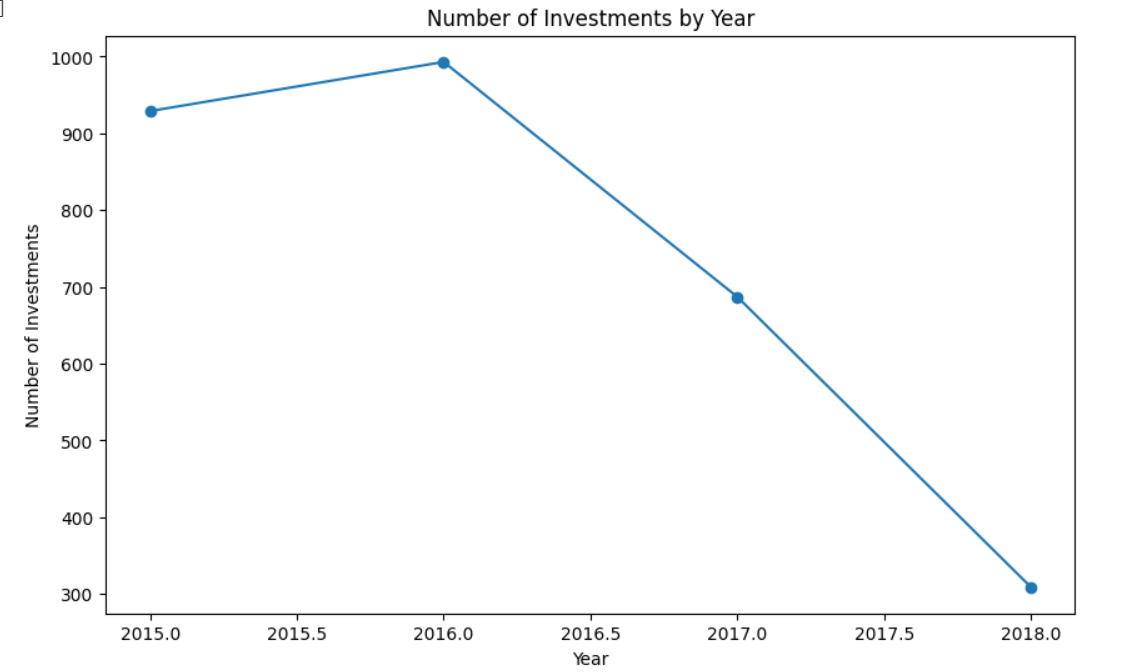
\includegraphics[width = 0.8\textwidth]{Figures/Pre_covid_Investments_Year.png}
    \caption{Investments made prior to COVID-19}
    \label{fig:Investments made prior to COVID-19}
\end{figure}

\subsection{Analysis of post-COVID funding data}

In the subsequent analysis phase, we begin by extracting raw data from a website's table format and storing it as a CSV file named "all\_tables\_data.csv". Post this, the dataset is cleaned to prevent any misinterpretation of data and saved into a new file "all\_tables\_data\_clean.csv" to serve as the basis for our analytical procedures.

After importing the new dataset, we employ the pandas library for visualization. We utilize the "head" function to initially observe dataset contents. Subsequently, we explore the data's shape and inspect column information. Proceeding to the data analysis stage, we identify prevalent sectors and depict this data through a pie chart.

Further insights are gained through a heatmap, enabling a comparison between geographical locations and startup stages. This heatmap provides valuable insights into the concentration of startup origins. By employing a categorical histogram function, we delve into the "Stage" column, revealing that a significant portion of startups underwent the Seed round.

In addition, a preliminary analysis of India's prime startup locations is presented through a bar graph. Employing various analytical processes, we aim to provide succinct yet informative conclusions derived from our data exploration. This multifaceted approach yields valuable insights into the dataset, ultimately contributing to a concise yet accurate analysis of the data.

\begin{figure}[ht]
    \centering
    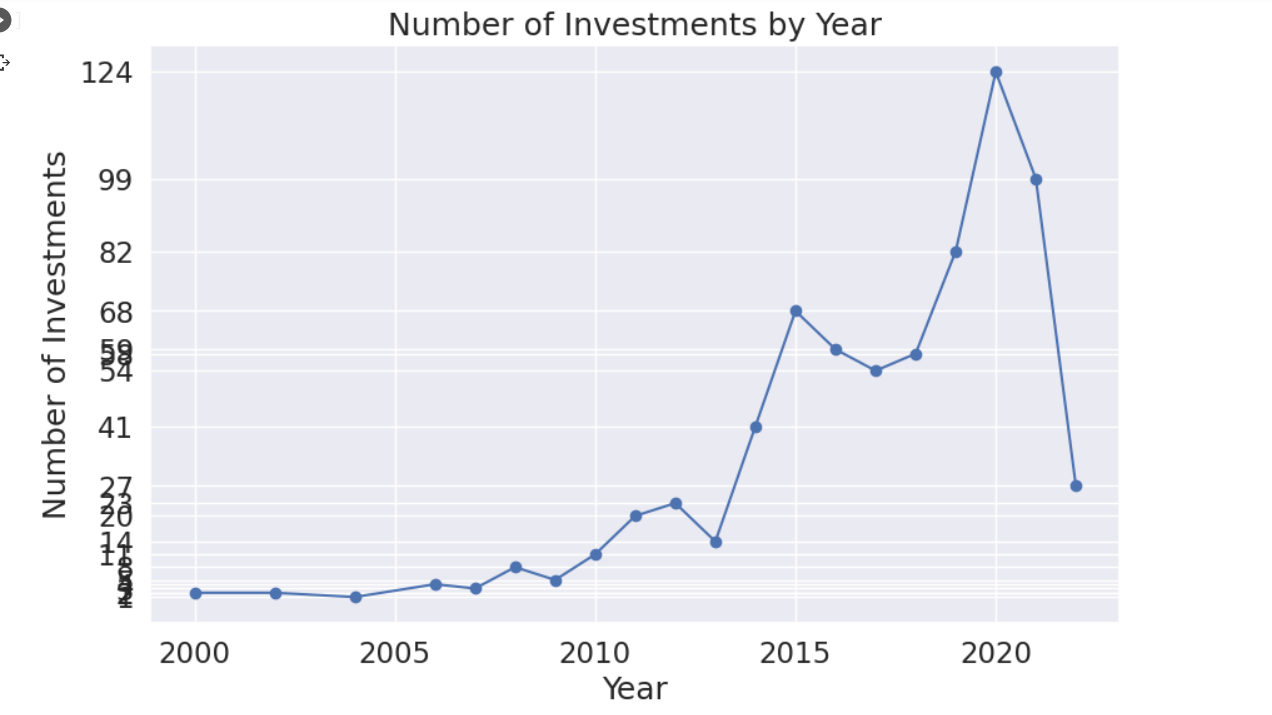
\includegraphics[width = 0.9\textwidth]{Figures/Post_covid_yearly_investments.png}
    \caption{Investments made post-COVID}
    \label{fig:Investments made post-COVID}
\end{figure}


\subsection{Data analysis strategy}

As already established, the projects deal with two kinds of datasets, one prior to a global crisis which is the pre-COVID era, and the other post the crisis, which is the post-COVID era distinguished based on years which serves as a crucial aspect for the analysis. Each of these datasets has to be handled differently based on their requirement which is further explained below.

\subsubsection{Pre-COVID analysis: Data Pre-processing}

Post successful data collection, the complete Dataframe is captured in a csv file 'startup\_funding.csv'.The initial step is to read the CSV file into the DataFrame using pd.read\_csv() function. Then, the code converts the Date "dd/mm/yyyy" column into a proper date format using the pd.to\_datetime() function which is able to, ensure compatibility with the "dd/mm/yyyy" format and also puts a check on the handling of the errors with the 'coerce' parameter.

The code then filters the DataFrame to include only rows where the "Date" falls within the years 2015 to 2018, then it stores the filtered data in the DataFrame `df\_pre`. Lastly, the filtered data is saved to a new CSV file named "startup\_data\_pre.csv" using `to\_csv()` without including the index column after that the dataset is now visualized by using the pandas library using the read functionality.

After getting the actual dataset that is required for analysis, the next step mainly focuses on preparing the data in a DataFrame which is named 'df\_pre' for analysis. It starts by identifying and counting all the null values that are present in each column of the DataFrame using the `isnull().sum()` function and then it displays the count. The code then focuses on the specific column which is named 'as Amount in USD'. Initially, this column is converted into a numeric format, and any of parsing errors are handled by coercing them into NaN values. The unique values which are present in the 'Amount in USD' column are printed, which mainly shows the presence of 'nan' (representing missing data) and the value is '4200000.0'. The code then proceeds to the further process where the 'Amount in USD' column is wrangled by removing all the commas from the values and then converting them into numeric format again. To address all the missing values in this column, the code then fills them with the median value of the 'Amount in USD' column. Now, the preprocessed DataFrame is saved as a CSV file named "startup\_data\_pre.csv".

\subsubsection{Pre-COVID analysis: Visualisation}

With data now preprocessed, it is ready for essential preliminary analysis. Initially, Python's Matplotlib library is leveraged to craft a bar plot portraying the dispersion of startups across distinct industry verticals. This entails computing the count of startups within each unique industry vertical from the 'df\_pre' DataFrame.

Following this, the ten industry verticals boasting the highest startup counts are singled out. Utilizing Matplotlib, a bar plot is generated. The x-axis denotes industry verticals, the y-axis signifies the corresponding startup numbers, and the bars illustrate startup frequency within each vertical. The plot is further enhanced with a title and axis labels: 'Industry Vertical' for the x-axis and 'Number of Startups' for the y-axis. Ultimately, the plot is exhibited using the plt.show() function. Similarly, multiple analyses and comparisons are visualized using matplotlib visualisation library. The top 10 investors are also calculated by summing up all the investments that are done by the investors and then they are compared with each other and a bar plot is used to visualize the comparison \citep{zhimeng2021assessing}. The same method is followed to visualise the top 10 locations within India where startups have been prevalent.

Moving on to important analysis, attention is directed toward visualizing the comprehensive investment trend analysis spanning multiple years. The Python code commences by segregating the investment data for meticulous analysis and visualization. This process initiates by extracting years from a DataFrame column denoted as 'Date' utilizing the .dt.year function.

Subsequently, the code tallies and computes investments for each year employing the value\_counts().sort\_index() function, ensuring comparison of occurrences across unique years arranged in ascending order. Employing the matplotlib library, a line plot is crafted. This plot illustrates investments on the y-axis vis-à-vis years on the x-axis. Circular markers denote data points. To enhance clarity, a title is appended, and the x-axis is labeled 'Year,' while the y-axis is labeled 'Number of Investments.' The visualization is ultimately displayed using plt.show().

The resulting visualization distinctly underscores the investment trend, revealing a substantial decline over the years. Notably, investments have witnessed a marked reduction throughout the pre-COVID period.

\begin{figure}[ht]
    \centering
    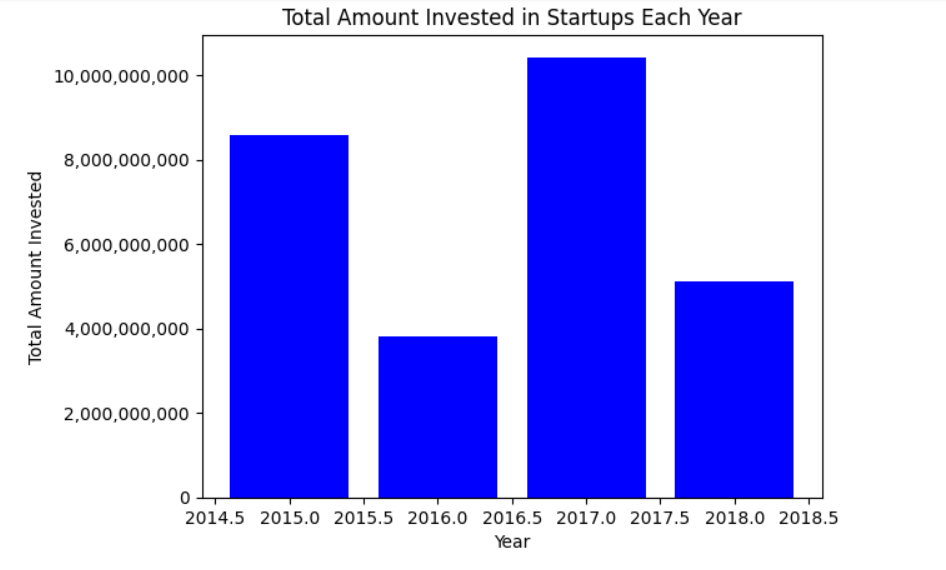
\includegraphics[width = 0.9\textwidth]{Figures/Pre_Covid_AmountInvested_Years.png}
    \caption{Amount invested prior to COVID}
    \label{fig:Amount invested prior to COVID}
\end{figure}


\subsubsection{Pre-COVID analysis: Machine Learning Algorithms}

The pivotal phase involves leveraging machine learning to derive insights from the comparison between independent and dependent values. Furthermore, it encompasses evaluating the precision and accuracy of the machine learning models incorporated in this analysis. Commencing this process, the Python libraries 'pandas' and 'scikit-learn' are harnessed to both preprocess and model the comprehensive startup data.
The initial steps entail importing essential modules requisite for data manipulation, preprocessing, and machine learning. Subsequently, data is loaded from the CSV file into a pandas DataFrame. Any vacant values within this DataFrame are addressed through substitution with empty strings. Categorical variables like 'city' and 'round' undergo conversion into numerical values using the LabelEncoder class. 'city' signifies distinct city names, whereas 'round' embodies cumulative funding across round types.
In this context, the independent variables (X) encompass 'round' and 'city,' while the dependent variable (y) encapsulates 'amount,' representative of total funding amounts. This dataset now serves as the foundation for training machine learning models, including the Support Vector Classifier (SVC). The performance of the model is gauged using the 'accuracy\_score' metric from 'scikit-learn.'
Overall, the code aims to acquire startup data for training a machine-learning model capable of predicting funding amounts based on funding round types and city locations.

After pre-training the dataset, the main performance analysis lies after the evaluation of the Support Vector Machine (SVM) model which is done through training the dataset. The dataset is now split into training and testing sets using an 80-20 ratio, where 80\% is used for training and 20\% for testing. The SVM model is first trained on the training data. After training, the model it is now able to make predictions on the test data. After the implementation of the model, the performance metrics are now calculated for the predicted results, the methods that are used are accuracy, precision, recall, F1 score, and a confusion matrix. Accuracy measures the percentage of correctly predicted instances. Precision is able to quantify the model's ability to correctly find the positive instance that is present among all the instances that are predicted as positive. Recall is used to measure the model's ability to correctly identify the positive instances that are present among all actual positive instances. F1 score is used to find the harmonic mean of the precision and recall, providing a balanced measure. The confusion matrix is used to display the counts of the true positive, true negative, false positive, and false negative predictions, which mainly offers insight into the model's performance for each of the classes. 'Weighted' averaging method is used for precision, recall, and F1 score, which accounts for class imbalance. Overall, the code assesses the SVM model's effectiveness in classification tasks and it provides a comprehensive view of its performance \citep{zhang2022startups}.

As the dataset is already split into training and testing sets using an 80-20 ratio, three other tree-based classification models as Decision Trees, Random Forests, and Extremely Randomized Trees are employed to further assist in the analysis. The models are then trained using the training dataset. Each of the models is initialized with a random state of 42 which is then used for reproducibility. After training, the predictions are then made on the testing data using each of the models separately. These predictions are then stored in `y\_pred\_dt`, `y\_pred\_rf`, and `y\_pred\_et` variables for the Decision Trees, Random Forests, and Extremely Randomized Trees, respectively. The results can be further evaluated and compared based on the performance of these tree-based models on the test data so that it is able to determine how well these models have performed.

Next, a function named evaluate\_model is defined, capable of accepting inputs such as the implemented machine learning model's name, actual labels y\_test, and predicted labels y\_pred. Within the function, it computes and presents diverse evaluation metrics aimed at gauging the model's performance on the provided data. These metrics encompass accuracy, precision, recall, and F1 score—widely recognized measures for assessing a classification model's prediction quality. This set of metrics mirrors those utilized to evaluate the SVM model's performance. Upon execution, the code showcases the confusion matrix, furnishing an intricate insight into the model's predictions across distinct classes. The function is subsequently employed to assess and exhibit all these metrics for four distinct models: Decision Trees, Random Forests, Extremely Randomized Trees, and Neural Networks. The overarching objective involves comparing and comprehending the performance of each model concerning the test data.

After that, a visual representation is created to demonstrate the comparison between all of the models. This makes it easier to evaluate each model's overall effectiveness on the dataset and enables efficient comparison and evaluation. The entire set of comparisons is provided in the section that follows for reference.


\begin{figure}[ht]
    \centering
    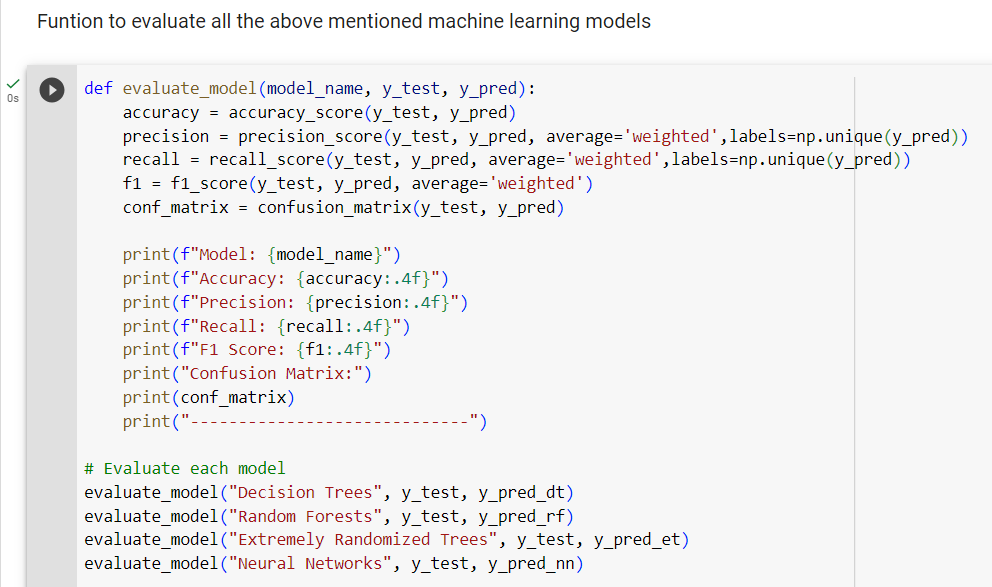
\includegraphics[width = 0.9\textwidth]{Figures/Evaluate_model.png}
    \caption{A common function used to evaluate all the models used}
    \label{fig:A common function used to evaluate all the models used}
\end{figure}

From, all the below visualisations it could be inferred that the Neural Networks Model has performed the best in accordance with the overall performance of all the models that have been used in this part of the analysis process.

\newpage
\begin{figure}[ht]
    \centering
    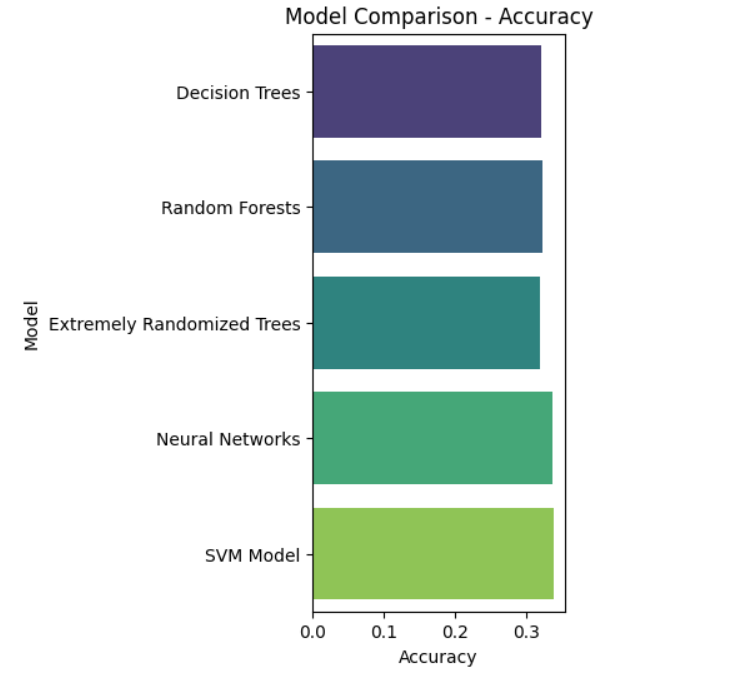
\includegraphics[width = 0.6\textwidth]{Figures/Pre_covid_Accuracy.png}
    \caption{Comparision of Accuracy among models for pre-COVID data}
    \label{fig:Comparision of Accuracy among models for pre-COVID data}
\end{figure}

\bigbreak

\begin{figure}[ht]
    \centering
    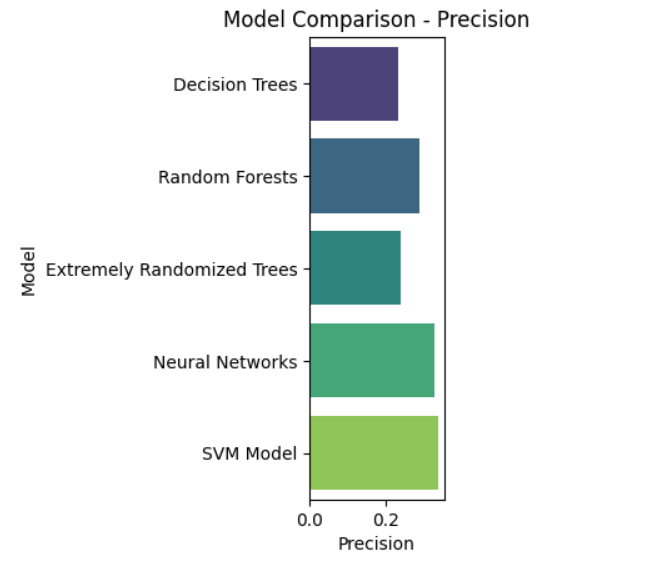
\includegraphics[width = 0.5\textwidth]{Figures/Pre_covid_Precision.png}
    \caption{Comparision of Precision among models for pre-COVID data}
    \label{fig:Comparision of Precision among models for pre-COVID data}
\end{figure}

\newpage
\subsubsection{Post-COVID analysis}

In this phase of analysis, the initial step involves scraping data from the website, followed by saving it into a fresh dataset. This dataset is then read using the pandas library, and its contents are visualized in the form of a dataframe. Before proceeding with data pre-processing, the commands df.info and df.shape are employed to determine the dataset's overall dimensions. Additionally, the df.info function is utilized to ascertain the total count of null values present in the dataset across all columns.

After identifying the count of null values, the next step involves preparing the dataset for machine learning models through comprehensive data wrangling. Before initiating the overall data-wrangling process, a preliminary analysis is conducted. This includes identifying the top 10 startup sectors. This involves gathering the necessary data and computing the distribution of all startups among these sectors in terms of percentage shares. This comparison is then visually represented using a pie chart, which displays the data proportions in terms of percentages. This process is performed to understand and get a visual representation of the data in hand.Various analyses were conducted to explore the relationships between different data fields within the dataset. Among these, a crucial analysis was focused on establishing a connection between startup funding and individual startups. The findings revealed that a substantial number of startups secured funding exceeding 200 million dollars. Notably, there was a significant upward trend in overall funding, signifying an increase in financial support for startups.

The code developed for analysing the post-pandemic data handles data pre-processing and machine learning tasks using the Pandas library and scikit-learn (sklearn) toolkit. Initial steps involve importing essential modules for data manipulation, data splitting, label encoding, SVM model application, and accuracy assessment. The script loads data from the 'all\_tables\_data.csv' CSV file into a Pandas DataFrame and addresses missing values by substituting them with empty strings. Categorical variables ('Sector' and 'Stage') undergo conversion into numerical values via the LabelEncoder. The 'Sector' and 'Stage' columns transform into their respective numerical representations. Independent features (X) consist of 'Stage' and 'Sector', while the dependent variable (y) is set as 'Amount'. This code's purpose is to prepare data for potential SVM classification, where 'Stage' and 'Sector' predict 'Amount', and model accuracy is evaluated using the accuracy\_score function.

The dataset is divided into training and test sets with an 80-20 split, allocating 80\% for training and 20\% for testing. Similar to the previous analysis, the SVM model is employed, and accuracy is computed using the confusion matrix. Similarly, the other three models—Decision Tree, Random Forest, Extremely Randomized Tree, Neural Networks (Multi-Layer Perceptron), and Gradient Tree Boosting—are also applied. Their accuracy metrics are compared and visualized as shown below. From the comparison, it is evident that Random Forest algorithms provides promising results.

\begin{figure}[ht]
    \centering
    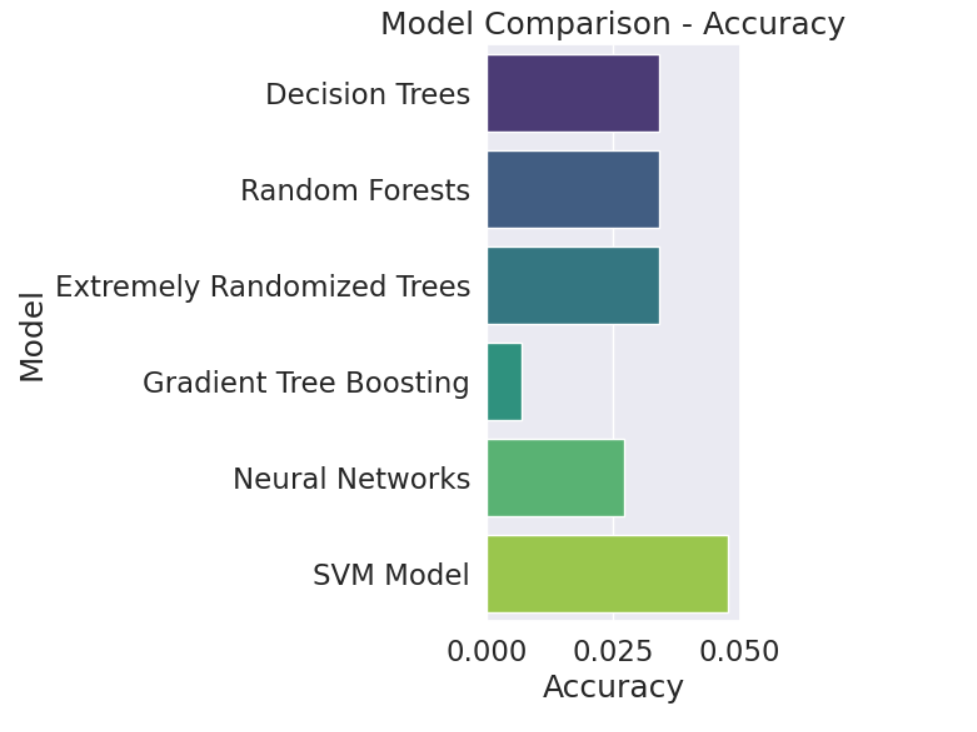
\includegraphics[width = 0.6\textwidth]{Figures/Post_covid_Accuracy.png}
    \caption{Comparision of Accuracy among models for post-COVID data}
    \label{fig:Comparision of Accuracy among models for post-COVID data}
\end{figure}

\bigbreak

\begin{figure}[ht]
    \centering
    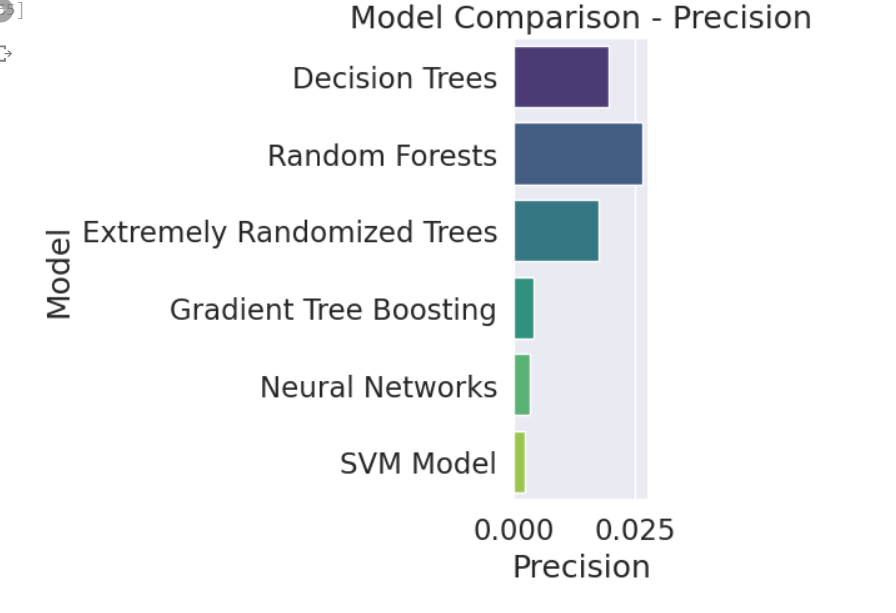
\includegraphics[width = 0.6\textwidth]{Figures/Post_covid_precision.png}
    \caption{Comparision of Precision among models for post-COVID data}
    \label{fig:Comparision of Precision among models for post-COVID data}
\end{figure}

\newpage
\subsection{EVALUATION}

\subsubsection{Chapter Overview}
In this section, the research question posited at the beginning of the study is reviewed, and the findings are evaluated.

\subsubsection{Research Questions}

\begin{enumerate}
    \item Can machine learning models get employed to make a prediction on the success rate of startups in India and check their ability to survive a global crisis like the COVID-19 pandemic or economic recession? 

    Given the limited size of the dataset at hand, Neural Networks demonstrated superior accuracy in comparison to alternative algorithms, particularly concerning the pre-COVID data. The neural networks' performance gain can be attributed to the ample size of the pre-COVID dataset, which contributed to their efficacy when contrasted with competing algorithms. Upon verifying different prediction parameters, it becomes evident that neural networks showcased commendable performance. But with post-covid data, Random Forests performed much better as seen by the model comparisons.

    \item How much has the COVID-19 pandemic contributed to the growth of startups in India, as measured by the percentage increase in the total funding raised by startups during the pandemic compared to the previous years?

    Analyzing the information and looking closely at the graphs showing the correlation between the years and related investments reveals a clear pattern. In the years before the COVID-19 pandemic began, investments made in the top 10 sectors show a progressive decline. In particular, investments fell significantly in 2018, and then barely any investments were made in 2019. The following years, however, show a divergent movement that illustrates an increase in investment levels. Notably, the year 2021 saw a significant increase in investments, indicating a promising future.
    
\end{enumerate}

\newpage
\section{DISCUSSION}
\subsubsection{Chapter Overview}

This chapter explores the numerous findings and observations made throughout the research as well as any potential obstacles that may have prevented the study from reaching its full potential.

\subsubsection{Observations of the study}

1. Pre-Covid Trends

The graph depicting investments displayed a consistent decrease leading up to the COVID-19 outbreak. This suggests that there was a prevalent pattern of declining investments during the designated timeframe prior to the pandemic. Multiple factors, such as the overall economic condition, prevailing market sentiment, business performance, and geopolitical occurrences, could have played a role in driving this decline.


2. Post-Covid Trends

Nonetheless, the landscape shifted considerably after the onset of the COVID-19 pandemic. The investment trend took a substantial turn in the post-COVID period, exhibiting a notable surge. This shift implies that after the pandemic, there was a pronounced increase in investment activities. Multiple factors could account for this upswing. For instance, governments and central banks globally implemented diverse fiscal and monetary policies to stimulate economic revival, potentially fostering greater investment engagement. Additionally, alterations in consumer patterns, advancements in specific sectors such as technology and healthcare, and broader market dynamics might have also contributed to this transformation.

By incorporating machine learning into this study, it may have been possible to move away from purely depending on subjective judgments and toward insights obtained from data-driven studies. Latent patterns, correlations, and associations that conventional statistical methods might miss are frequently present in large datasets. These hidden elements can be revealed via machine learning methods. It is important to recognize that while the research offers insights based on data that is currently accessible, it may not fully reflect all the nuances of the investment landscape. Furthermore, the quality of the data and its ability to accurately reflect the larger environment, together with the specific qualities and algorithms included in the machine learning framework, all have a significant role in how accurate the results of such investigations are.

\subsubsection{Limitations of the study}

The pursuit of predicting startup success through machine learning encounters a realm of challenges that emphasize the intricate nature of the startup ecosystem. While machine learning offers a data-driven lens, it's essential to acknowledge the boundaries within which these predictive models operate.

A primary constraint revolves around the availability and quality of data. For machine learning to thrive, it demands an ample and robust dataset. Startups, especially those in their infancy, might not possess extensive historical data essential for comprehensive analysis. In turn, this issue can hinder the model's capacity to discern long-term trends and patterns.

The dynamic environment within which startups operate introduces a layer of uncertainty. The startup landscape is marked by its rapid evolution, where market dynamics, consumer preferences, and industry trends are prone to swift and unforeseen shifts. Such dynamism challenges, the relevance of historical data as a basis for prediction in a rapidly transforming context.On going through the dataset and performing analyses during the study, it was evident that there are factors like innovation and adaptability that the startups had incorporated which probably helped them thrive during the pandemic. Much investigation and research have to be made on how to utilise innovation as a parameter in the success prediction of startups.

\newpage
\section{CONCLUSION}
\subsubsection{Chapter Overview}

This chapter details all the observations that have been noticed throughout the study and suggests the necessary future course of action that can be pursued.

\subsubsection{Summary}

Predicting a result in any situation is challenging, especially when there are dynamic aspects involved, but estimating the success rate of startups in a developing nation like India is unquestionably a tremendous responsibility. But we can make it happen with the aid of innovations like machine learning. Even if we are able to anticipate a startup's success using the apparent indicators, there will always be an unnoticed component that could drastically alter our assessment. One such is a global crisis. Pandemics, war, and other crises like the recession strike suddenly. Consequently, including the variables for a crisis seems like a reach, but it is a safe and prudent choice. We became much more aware of how unprepared we are as a result of the COVID-19 outbreak. While some firms that only operated online were able to adjust and survive, many of them failed. Although government initiatives were taken to nurture the startup environment, the turbulent environment during the pandemic caused some major fluctuations as witnessed by the study.

\subsubsection{Inference}

The central focus of the study was to employ advanced machine learning algorithms to forecast the likelihood of success for startups operating within India's entrepreneurial landscape. Moreover, the study sought to delve into the startups' capabilities to withstand challenging circumstances, particularly in the context of the COVID-19 pandemic. Additionally, the study aimed to identify the specific attributes that contributed to the resilience of these startups during times of crisis. To accomplish these objectives, an extensive dataset was meticulously curated through a comprehensive review of relevant literature. This dataset was meticulously categorized into two distinct segments: the pre-COVID era and the post-COVID period. This categorization aimed to enable a clear distinction between the periods and facilitate an in-depth analysis of the data. Subsequently, an array of rigorous analyses were conducted, employing six distinct machine learning algorithms. Among the various algorithms utilized, Neural Networks and Random Forest models emerged as notable frontrunners. These models showcased remarkable performance in terms of accuracy and precision compared to their counterparts despite the smaller dataset. Furthermore, the study underscored the essential role played by financial investments and funding in shaping startup resilience, as exemplified by the sustained increase in investments following the pandemic's wake and also the post-pandemic years.

\subsubsection{Ethical Considerations}

Upholding ethical principles is still essential when using publicly accessible data. The dataset used in this study contains actual data on funding for various businesses over a range of periods of time and locations. The dataset also includes information about the investors and founders of these firms. Careful attention was paid to prevent any unauthorized exposure, misuse, or manipulation of the data in order to preserve the integrity and privacy of this information. Throughout the course of this study, All efforts were made to ensure that the data was treated with the highest care and sensitivity.

\subsubsection{Future Works}

While machine learning offers a promising avenue for understanding startup success, it must be approached cautiously and balanced with the awareness of its limitations. A holistic view of the startup ecosystem demands integration with human expertise, nuanced understanding, and consideration of dynamic factors that extend beyond data analytics. Predicting startup success necessitates navigating a landscape where data-driven insights coalesce with contextual understanding to unveil a comprehensive picture.
In Addition, the analyses performed here could serve as a basis for understanding a fast-growing startup also known as "unicorns" \citep{rodrigues2021companies}.

The examination of these findings holds the potential to offer valuable insights to both entrepreneurs and investors alike, providing them with a clearer comprehension of the market dynamics and the ability of their startups to endure fluctuations within the industry. Moreover, the outcomes of this study underscore the significance of an Initial Public Offering (IPO) for startups seeking legitimacy and resources \citep{lee2008strategy}. Going public through an IPO enables startups to gain access to substantial capital infusion, paving the way for their expansion, innovation, and long-term sustainability. 


%TC:ignore
\pagebreak
\bibliography{References}
%TC:endignore

\end{document}
